\documentclass[../preview.tex]{subfiles}
\begin{document} 
\begin{figure}
\centering
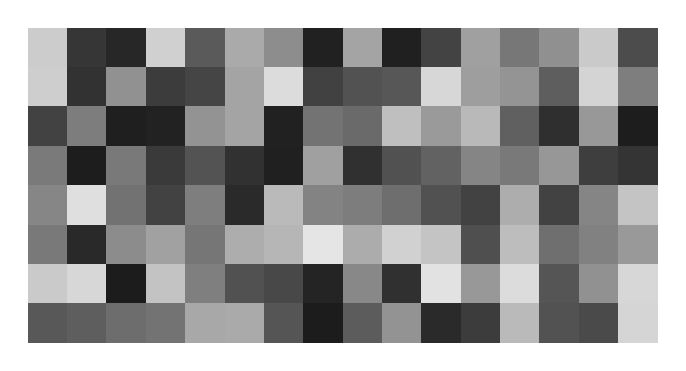
\begin{tikzpicture}[scale=0.5]
\pgfmathsetmacro {\N }{8}
\pgfmathtruncatemacro {\Na }{\N -1}
\pgfmathsetmacro {\D }{16}
\pgfmathtruncatemacro {\Da }{\D -1}
%\draw (0, 0) grid (8, 4);
\foreach \r in {0,...,\Na}{
    \foreach \c in {0,...,\Da}{
        \pgfmathparse{0.8*rnd+0.1};
        \definecolor{MyColor}{rgb}{\pgfmathresult,\pgfmathresult,\pgfmathresult}
        \fill[fill=MyColor] (\c, \r) rectangle (\c+1,\r+1);
    }
}
\end{tikzpicture}
\end{figure}
\end{document}
